        \clearpage
        \begin{figure*}[ht]
            \pdfbookmark[2]{ID 07}{figure_id_07}
        	\centering
            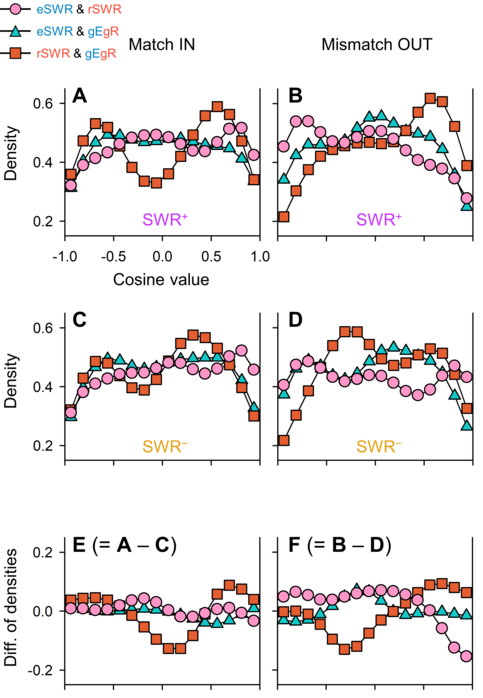
\includegraphics[width=0.5\textwidth]{./src/figures/.png/Figure_ID_07.png}
        	\caption{\textbf{
Direction of Neural Trajectory During SWR Based on Encoding and Retrieval States
}
\smallskip
\\
\textbf{\textit{A--B}} The kernel density estimation distributions of $\protect\overrightarrow{{\mathrm{eSWR^+}}}$ $\cdot$ $\protect\overrightarrow{{\mathrm{rSWR^+}}}$ (\textit{pink circles}), $\protect\overrightarrow{{\mathrm{eSWR^+}}}$ $\cdot$ $\protect\overrightarrow{{\mathrm{g_{E}g_{R}}}}$ (\textit{blue triangles}), and $\protect\overrightarrow{{\mathrm{rSWR^+}}}$ $\cdot$ $\protect\overrightarrow{{\mathrm{g_{E}g_{R}}}}$ (\textit{red rectangles}) in Match In (\textit{A}) and Mismatch OUT tasks (\textit{B}). \textbf{\textit{C--D}} The corresponding distributions of $\mathrm{SWR^-}$ instead of those of $\mathrm{SWR^+}$ in \textit{A} and \textit{B}. \textbf{\textit{E--F}} The differences in the distributions of $\mathrm{SWR^+}$ and those of $\mathrm{SWR^-}$, showing SWR components (\textit{E} = \textit{C} - \textit{A} \& \textit{F} = \textit{D} - \textit{B}). Biphasic distributions of $\protect\overrightarrow{{\mathrm{rSWR^-}}}$ $\cdot$ $\protect\overrightarrow{{\mathrm{g_{E}g_{R}}}}$ indicate fluctuations between the encoding and retrieval states during the Sternberg task. Also, contradicting directionality between $\protect\overrightarrow{{\mathrm{eSWR^+}}}$ and $\protect\overrightarrow{{\mathrm{rSWR^+}}}$ was observed (pink circles) not in Match IN task (\textbf{\textit{E}}), but in Mismatch OUT task (\textbf{\textit{F}}). Lastly, transitions from the retrieval to encoding states are evident in the SWR components in both Match IN and Mismatch OUT tasks (\textit{red rectangles} in \textit{E--F}).
}
% width=0.5\textwidth
        	\label{fig:07}
        \end{figure*}
